\section{Limitazione Accesso}
Utilizzando i router in Cisco packet tracer abbiamo visto tre modalità differenti di questi, ognuna permette l’utilizzo di comandi unici, che in altre modalità non funzionerebbero, queste tre modalità sono la user mode, la privileged mode e la configuration mode.

\subsection{Modalità di esecuzione dei comandi}
Nello schema sottostante è rappresentata la gerarchia delle modalità e alcuni comandi di esse

\begin{center}
    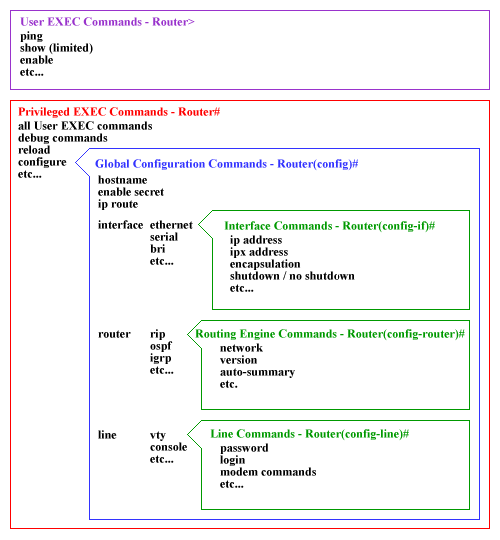
\includegraphics[width=0.9\textwidth]{images/03.limitazione.accesso/01.exec-modes.png}
\end{center}

\subsubsection{User mode}
La user mode è la prima modalità a cui un utente ha accesso dopo aver effettuato l’accesso al router. La user mode può essere identificata dal prompt> che segue il nome del router. Questa modalità consente all’utente di eseguire solo i comandi di base, come quelli che mostrano lo stato del sistema. Il router non può essere configurato o riavviato da questa modalità.

La user mode può essere identificata con \emph{Hostname>}

\subsubsection{Privileged mode}
La modalità privileged mode consente agli utenti di visualizzare la configurazione del sistema, riavviare il sistema e accedere alla modalità di configurazione del router. La privileged mode consente anche tutti i comandi disponibili nella user mode. La privileged mode può essere identificata dal prompt \# che segue il nome del router. Dalla user mode, un utente può passare alla privileged mode, eseguendo il comando “enable”. È possibile impostare una password per accedere a questa sezione.

La privileged mode può essere identificata con \emph{Hostname\#}

\subsubsection{Configuration mode}
La configuraion mode globale consente agli utenti di modificare la configurazione del sistema in esecuzione. Dalla privileged mode un utente può passare alla configuration mode eseguendo il comando “configure terminal” dalla privileged mode. Per uscire dalla configuration mode, l’utente può immettere il comando “end” o premere la combinazione di tasti Ctrl-Z.

La configuration mode  globale può essere identificata con \emph{Hostname (config) \#}

La configuration mode globale ha varie sottomodalità, a partire dalla configuration mode globale, che può essere identificata dal prompt (config) \# dopo il nome del router. Di seguito sono riportate le importanti sottomodalità di configurazione globale.

\begin{itemize}
    \item Interface mode: modalità di configurazione dell’interfaccia fisica del router. Indentificata con \emph{Hostname (config-if) \#}
    \item Line mode: modalità di configurazione della linea del router – console, vty ecc. Identificata con \emph{Hostname (config-line) \#}
    \item Router configuration mode: modalità di configurazione dei protocolli di routing. Identificata con \emph{Hostname (config-router) \#}
\end{itemize}

\subsection{Password}
Diversi tipi di password possono essere configurate su un router Cisco, come la password di abilitazione, la password segreta e anche la porta della console. Tutte queste posizioni delle password rappresentano buone posizioni di accesso per le password, ma se hai solo una password su una sola posizione di accesso, dovresti almeno avere una password di abilitazione.

\subsubsection{Enable}
La password di abilitazione viene utilizzata ogni volta che si passa dalla EXEC user mode alla EXEC privileged mode. Questa password ti dà sicurezza sul tuo router perché la Privileged mode EXEC è dove si trovano tutti i comandi pericolosi, incluso l’accesso alla modalità Configurazione globale. Per impostare una password di abilitazione, si utilizza il Comando~\ref{cmd:set-pwd}

\begin{cmds}{Configuration mode}{cmd:set-pwd}{Assegnazione della password di abilitazione}
    \$ enable password \textcolor{Highlight1}{mypassword}
\end{cmds}

La password tuttavia viene memorizzata nel file di configurazione in chiaro (visibile con i Comandi~\ref{cmd:see-pwd}), quindi chiunque abbia accesso al file di configurazione potrebbe decidere di leggere la password.

\begin{cmds}{Configuration mode}{cmd:see-pwd}{Estrapolare la password di attivazione dal file di configurazione}
    \$ show running-config | include enable password
\end{cmds}

\subsubsection{Secret password}
La soluzione di Cisco al problema intrinseco della password di abilitazione consiste nel creare un nuovo tipo di password chiamata password segreta. La password segreta sositutisce l'enable password e verrà utilizzata per passare dalla User mode alla Privileged mode. Per impostarla è sufficiente utilizzare il comando~\ref{cmd:secret-pwd}

\begin{cmds}{Configuration mode}{cmd:secret-pwd}{Impostare la password segreta}
    \$ enable secret \textcolor{Highlight1}{miapassword}
\end{cmds}

Se si prova a leggere la password dalla configurazione si ottiene una stringa cifrata come ``enable secret 5 \$1\$BSX4\$FZp.ZFvYSAGUEDn8dvr140''

\subsubsection{Console}
I dispositivi di rete Cisco utilizzano le parole per fare riferimento ai componenti software che gestiscono le sessioni CLI locali e remote. Utilizzare il comando dalla configurazione globale della line console 0 per accedere alla modalità di configurazione della riga per configurare le opzioni, come una password, per la porta della console.

\begin{cmds}{Configuration mode}{cmd:set-console-pwd}{Impostare la password console}
    \$ line console 0\\
    \$ password \textcolor{Highlight1}{mypassword}
\end{cmds}

\subsubsection{Remote}
Le sessioni CLI remote utilizzano linee che si riferiscono a linee di telescrittura virtuale (VTY). Si usa il comando in configurazione globale line vty numero riga [numero riga finale] per accedere alla modalità di config-line per configurare le opzioni, come una password, per le sessioni CLI remote

\begin{cmds}{Configuration mode}{cmd:set-remote-pwd}{Impostare la password per connessioni remote come Telnet e SSH}
    \$ line vty 0 4\\
    \$ password \textcolor{Highlight1}{mypassword}
\end{cmds}

\subsection{Message of the Day}
I banner sono messaggi visualizzati agli utenti che si connettono ai router tramite le varie linee (console, vty e ausiliaria). I banner vengono solitamente utilizzati per visualizzare un messaggio che vieta l’accesso non autorizzato e per avvisare delle conseguenze legali in caso di infrazione. Per impostare il messaggio del giorno si possono usare i comandi nel blocco~\ref{cmd:set-motd}

\begin{cmds}{Configuration mode}{cmd:set-motd}{Impostare il \textcolor{Highlight3}{messaggio del giorno}, viene delimitato dai due \textcolor{Highlight2}{caratteri} all'inizio e alla fine.}
    \$ banner motd \textcolor{Highlight2}{\#}\textcolor{Highlight3}{Authorized Personnel Only}\textcolor{Highlight2}{\#}
\end{cmds}
